\documentclass{article}
\usepackage{parskip}
\usepackage{pdfpages}
\usepackage[margin=.6in]{geometry}
\begin{document}
\includepdf[pages=2]{slides}
There is time asymetry with how energy works. For instance dropping an egg can only go one direction.

\includepdf[pages=3]{slides}
We start with a hot up of coffee with lots of thermal energy. We leave it to sit for a while and it starts passing its thermal energy to the air around it. So we have concentrated energy spontaneously disperse, but we never see the opposite happen. This is called entropy.

\includepdf[pages=4-5]{slides}
Brownian motion was used as proof fro democratus's ideas.

\includepdf[pages=7]{slides}
Diffusion is the migration of particles from high concentration to a region of low concentration. This happens randomly without outside influence.

\includepdf[pages=8]{slides}
All motion is random. So we look at the average particles. Say we divide some water into cross sections. We can say that on average half of the particles in one section will move right and half will move left. This results in this diffusion of particles from high to low concentration. From this we can derive a law which is boss.

\includepdf[pages=9]{slides}
The end result of diffusion is a dynamic equilibrium because shits still moving but a balance has been reached.

\includepdf[pages=10]{slides}
Nature does not prefer an spread out of dye molcules in water. It really doesn't care. Its basically just a probabilty thing. There are way more possibilities that have more spread out particles rather than clumps.

\includepdf[pages=11]{slides}
There si random jiggling of water molecules which is held over from the big band theory. These water molecules collide with the dye molecules. These move things around. Statistically speaking it is nearly guarenteed that the mixture will end up looking homogeneous.

Our body is very good at extracting order from the things we consume. So basically we are reversing the diffusion process.

\includepdf[pages=12]{slides}
The diffusion process defined above also applies to the energy in a coffee cup. We call this law of diffusion the second law of thermal dynamics.

\includepdf[pages=13]{slides}
Basically the second law of thermal dynamics is that energy tends to spread out. Entropy is kind of a measure of disorder. It is possible to have places in the universe where entropy is decreasing, but you will always have a net positive growth of entropy.

What animates us is random thermal motion left over from the big bang which our body extracts order from and uses to move.

\includepdf[pages=14]{slides}
\includepdf[pages=15]{slides}
Entropy was first denoted with S. It stated around the time people wanted to make steam engines more efficient. The energy flowing from the hot object to the cold object divided by the temperature. Doing this for the hot object and the cold object are not equal (they sum to a non zero value). When you add them you get a positive value. This means that the cold object has more entropy.

This lead us to know that the amount of entropy is always increasing.

\includepdf[pages=16]{slides}
The equation $S=k\log W$ gives us a great understanding of entropy.

\includepdf[pages=17]{slides}
A water droplet has a fairly high level of disorder (many ways to arrange them and have it look the same), but when we freeze it there is much less disorder (fewer ways for it to be arrange).

\includepdf[pages=18]{slides}
Crystal structures have some order, but you can rearrange them alot. But if you try to do the same with dna lots of shit changes. So we can say that dna is highly ordered.

\includepdf[pages=19]{slides}
$S=k\log W$

K is Boltzmann's constant. For the sake of understanding we are just going to ignore this, its a constant, who cares. W is the number of microstates compatible with a given macrostate.

\includepdf[pages=20]{slides}
Take a balloon for example. We can describe its macrostate using a few parameters (volume, temperature, pressure). The microstate however is determined on the position, and velocity of every air molecule.

\includepdf[pages=21-29]{slides}
There is a point at which the temperature of the system is the same as its environment. At this point equilibrium has been reached. No more diffusion then.

\includepdf[pages=30-41]{slides}
Theres an argument that life violates the second law of thermal dynamics because entropy goes down in cells. This is actually fine, there is nothing that says entropy can never go down, just that its net is increasing. Similar arguments are made for evolution which is dumb.

Yeah, at this point I totally stopped paying attention. He just sorta continued rambling on about how entropy works. You got this future lara, I believe in you.

\includepdf[pages=42-76]{slides}

































\end{documents}
